\documentclass[article]{beamer}
\usetheme{Warsaw}
\setbeamertemplate{footline}[frame number]

\usefonttheme[]{serif}
\usepackage{amsmath, latexsym, color, graphicx, amssymb, bm, here}
\usepackage{epsf, epsfig, pifont,tikz,subfigure}
\usepackage{graphics, calrsfs}
\usepackage{times}
\usepackage{fancybox,calc}
\usepackage{palatino,mathpazo}
\usepackage{amsfonts}
\usepackage{sidecap}
\usepackage{listings}
\usepackage{hyperref}
\usepackage{algorithm, algorithmic}

\title{Graph Theory: Bellman-Ford}
\author{David Jacobo \\ \href{mailto:jguillen@cimat.mx}{jguillen@cimat.mx}}
\date{\scriptsize{\today}}

\AtBeginSection[]
{
  \begin{frame}{Outline}
    \tableofcontents[currentsection]
  \end{frame}
}

\begin{document}

%%%%%%%%%%%%%%%%%%%%%%%%%%%%%%
\maketitle			
			
%%%%%%%%%%%%%%%%%%%%%%%%%%%%%%
\begin{frame}
\frametitle{Definition}
\begin{center}
\huge
	G = (V, E)
	
\vspace{8mm}	
	
%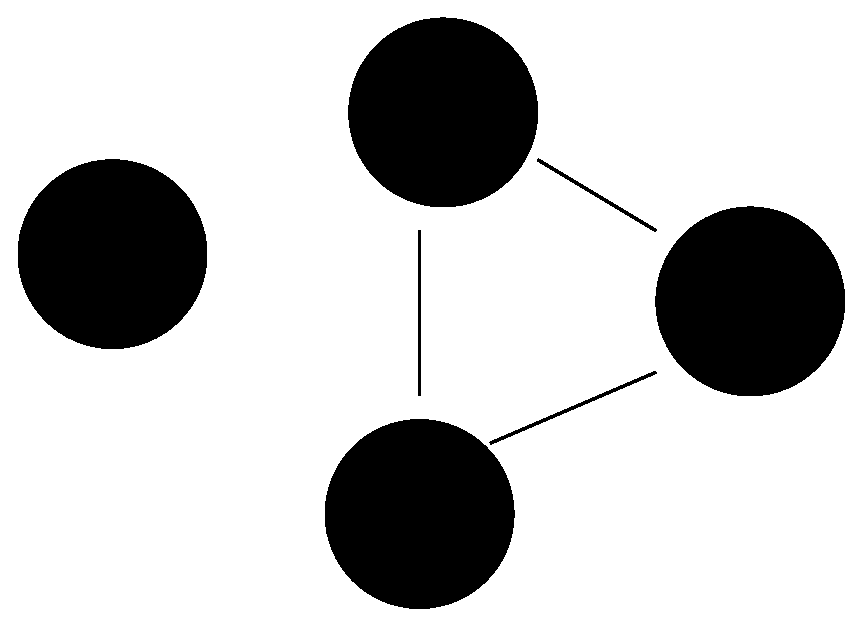
\includegraphics[scale=0.3]{./figures/graph.eps}
\end{center}
\end{frame}

\begin{frame}
\frametitle{Discussion}
\begin{center} 
Why aren't we able to solve \textbf{Single Source Shortest Paths (SSSP)} correctly with Dijkstra's algorithm under the presence of negative edges?
\end{center}
\end{frame}

%%%%%%%%%%%%%%%%%%%%%%%%%%%%%%

\section{SSSP w/ negative weights}
\subsection{Intuition}
\begin{frame}
	\frametitle{Intuition}
	
	Given a \textbf{weighted graph} and an initial vertex, \textbf{calculate the shortest paths to all the other vertices (SSSP)}. Report negative cycles if present and decide the vertices affected by those cycles

\end{frame}

\begin{frame}
	\frametitle{Algorithm}
	
		\begin{algorithm}[H]
		\begin{algorithmic}[1]			
		\FOR{$u$ $\in$ $V$ }
		\STATE $dist[u] = INF$
		\STATE $parent[u] = INV$
		\ENDFOR
		\STATE $dist[source] = 0$
		
		\end{algorithmic}
		\caption{Set initial distances}
		\label{alg:seq}
		\end{algorithm}	
	
\vspace{5mm}

Here INF is a pretty big value, how to choose it? do the math and watch for the largest possible value on your graph. INV is an INValid value, -1 on my code since we know our vertices are given in the range $[0,V-1]$	
	
\end{frame}
%%%%%%%%%%%%%%%%%%%%%%%%%%%%%%%%%

%%%%%%%%%%%%%%%%%%%%%%%%%%%%%%%
\subsection{Algorithm}
\begin{frame}
	\frametitle{Algorithm}
	
		\begin{algorithm}[H]
		\begin{algorithmic}[1]
		\FOR{i=0:v-1}
		\FOR{$u \forall V$}
		\FOR{$n:local-neighbours[u]$}
		\STATE $d = dist[u] + n_{w}$\
		\IF{$d < dist[n_{y}]$}
		\STATE $dist[n_{y}] = d$
		\STATE $parent[n_{y}] = u$
		\ENDIF
		\ENDFOR
		\ENDFOR
		\ENDFOR
		
		\end{algorithmic}
		\caption{Compute distances}
		\label{alg:seq}
		\end{algorithm}	
	
\end{frame}

\begin{frame}
	\frametitle{Algorithm}
	
		\begin{algorithm}[H]
		\begin{algorithmic}[1]
		\STATE Set initial distances
		\STATE Compute distances
		\STATE Call compute distances again, if a single value is updated then we have a negative cycle	
		\STATE Detect vertices which distance will keep decreasing forever $:'($ if needed	
		\end{algorithmic}
		\caption{Bellman-Ford}
		\label{alg:seq}
		\end{algorithm}	

\end{frame}

\subsection{Time/Memory complexity}
\begin{frame}
\textbf{Time complexity:} We are running the whole graph (V+E), V-1 times, plus a single run to watch for negative cycles, thus:

\vspace{5mm}

\begin{center} \textbf{$O(VE)$} \end{center}

\vspace{8mm}

\textbf{Memory complexity:} We need to keep track of the distances and parents per each vertex, so a linear amount of memory is needed with respect to $(w.r.t.)$ V:

\vspace{5mm}

\begin{center} \textbf{$O(V)$} \end{center}

\vspace{5mm}

This memory analysis doesn't take into account the space to save the graph (that's up to the problem requirement).
\end{frame}


\subsection{Tips and tricks}
\begin{frame}
	\frametitle{Keep in mind...}
	\begin{itemize}
		\item Use Bellman-Ford only if the graph is known to have negative edges.
		\item Remember this algorithm is for a Single Source, we will address the All Pairs Shortest Paths (APSP) later on.
		\item Relax is again the key component.
		\item Remember that the V-1 iterations are required because of the case when the given graph is a directed list.
	\end{itemize}
\end{frame}

%%%%%%%%%%%%%%%%%%%%%%%%%%%%%%
\begin{frame}[plain]
\frametitle{}
\begin{center}
\Huge{\color{blue}{Q \& A}} \\
\vspace{5mm}
%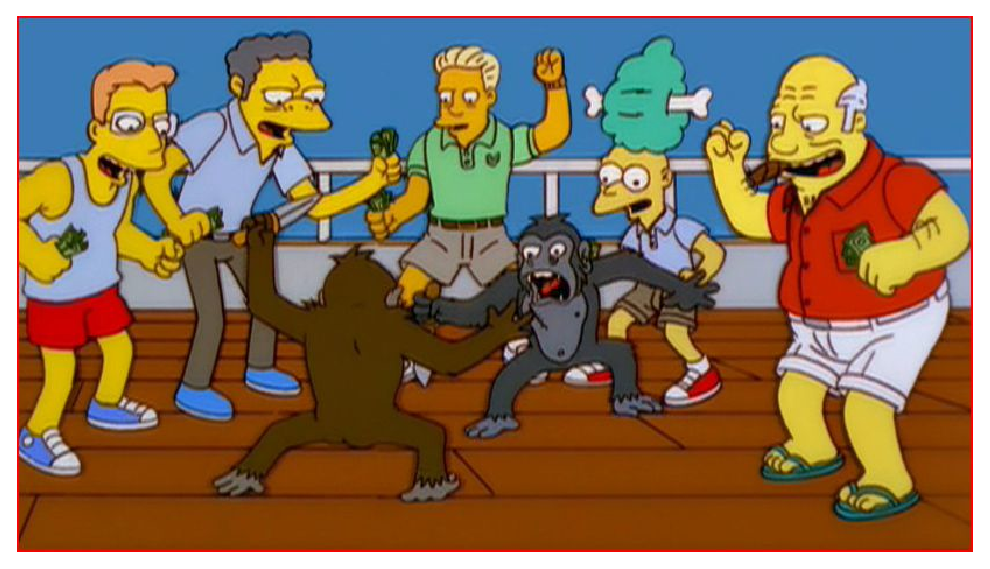
\includegraphics[scale=0.4]{./figures/monkey_fight.eps}
\end{center}
\end{frame}

%%%%%%%%%%%%%%%%%%%%%%%%%%%%%%%%
\begin{frame}[plain]
	\textbf{References}
	\begin{itemize}
		\item \href{https://sites.google.com/site/stevenhalim/}{Competitive Programming site}
		\item \href{https://github.com/davidjacobo/algorists/}{Algorists' repository}
	\end{itemize}
\end{frame}
\end{document}
